El filtro decode consiste en la decodificacion de un texto embebido en los bits menos significativos de los pixeles de una imagen. Cada 4 bytes, se toman los dos bits menos significativos de cada uno y se obtiene un nuevo byte que es la codificacion ascii de un caracter del texto. Tambien se utilizan el tercer y cuarto bit menos significativo de cada byte para saber como interpretar esos bits y aplicarles operaciones.
\par
\bigskip
Se implemento una primera version del algoritmo en C, analicemos el algoritmo y luego veamos que optimizaciones se le aplicaron.
\subsubsection{Descripcion del algoritmo}

\textbf{Nota: la idea de este codigo es entender como funciona nuestro algoritmo, por ello se eliminaron varias partes del codigo original.}\\
\lstinputlisting[language=C,tabsize=4, numbers=left, numberstyle=\tiny\color{black},mathescape=true, backgroundcolor=\color{gray}, rulecolor=\color{black}, keywordstyle=\color{blue}, commentstyle=\color{dkgreen},stringstyle=\color{mauve}, numbersep=5pt, basicstyle=\scriptsize]{fuentes/pseudodecode_c.c}
\textbf{Explicacion del algoritmo:}\\
Analicemos por partes que hace este algoritmo:\\
\begin{itemize}
    \item \textbf{Lectura de 4 bytes de origen:} Lineas 4-7\\
        En esta sección se leen de origen 4 bytes que contendrán en los 4 bits menos significativos de cada uno la informacion correspondiente a un char del mensaje codificado.
    \item \textbf{Filtrado con mascaras de valores relevantes:} Lineas 10-19\\
        Luego, debemos separar de alguna manera los bits que nos interesan del resto, para ello utilizamos mascaras de bits que por medio de operaciones logicas de conjuncion y corrimiento nos permiten quedarnos con los bits que nos interesan, en este caso code(primeros 2 bits) y op(tercer y cuatro bit).
    \item \textbf{Procesado del code segun el op:} Lineas 22-25\\
        Ya tenemos organizados los datos de las etapas anteriores de forma tal que podemos aplicar una serie de comparaciones al op para saber cual operacion realizarle al code correspondiente, para esto utilizamos una funcion auxiliar que nos devuelve el code listo para ser combinado.
    \item \textbf{Combinacion y escritura a destino:} Lineas 28-30\\
        Tal como dice el enunciado, realizamos un mezclado de los 4 bytes(notar que solo se utilizan 2 bits de cada uno) por medio de corrimientos y operaciones logicas de disyuncion. De esta forma hemos armado un caracter del mensaje, el cual es escrito al buffer de salida pasado por parametro.
\end{itemize}
\bigskip
\textbf{Optimizaciones realizadas:}
\begin{itemize}
    \item \textbf{Eliminacion de la llamada a la funcion auxiliar por medio de modificador inline:}\\
        De esta forma, con este modificador pretendemos eliminar los saltos de la llamada a funcion, requiriendole al compilador introducir el cuerpo de la funcion en cada invocacion a esta.
\end{itemize}

\bigskip
\textbf{Detalles de implementacion:}
\begin{itemize}
    \item \textbf{Multiplicidad de la cantidad de bytes a procesar:}\\
        En nuestra implementacion no tuvimos en cuenta el caso donde la cantidad de bytes a procesar no es multiplo de 16, es decir, que el ultimo ciclo, leeria memoria invalida al introducir una entrada que no respete esta precondicion de multiplicidad de tamaño.Para solucionarlo se podria implementar una solucion que consiste en iterar sobre los primeros k-bytes tal que k sea el primer multiplo de 16 hacia menos infinito. y luego, fuera de dicho ciclo, restarle al puntero 16 menos el resto modulo 16 del tamaño de la entrada y hacer un salto no condicional al comienzo del ciclo, luego de ejecutarse una vez mas, automaticamente la guarda se vuelve falsa y termina el ciclo.
\end{itemize}

\subsubsection{Implementacion en assembler utilizando set de instrucciones SIMD}

Luego de realizar la anterior implementacion en C, nos pusimos a pensar la mejor manera de utilizar SIMD con el set de instrucciones que teniamos a nuestro alcance.
Consideramos realizar la implementacion en assembler con la ventaja de poder utilizar los registros XMM de un tamaño de 16 bytes y maximizar su capacidad para leer mas de 4 bytes en cada ciclo. Dicho esto, la version en assembler obtiene 16 bytes por ciclo, y con las instrucciones de operatorias empaquetadas se espera procesar 4 veces mas datos por ciclo.\\
\\
\textbf{Nota: } En esta implementacion nos dimos cuenta que en muchos lugares utilizamos unicamente 2 bits de los 16 bytes empaquetados, pero dadas las instrucciones a nuestro alcance, consideramos que es la mejor implementacion en SIMD respetando un balance entre el set de instrucciones a nuestro alcance y el rendimiento.

\subsubsection{Analisis}
Antes de comenzar el ciclo principal nos vimos con la necesidad de declarar algunas mascaras como variables globales inicializadas para la manipulacion de los bits, y las cargamos en registros XMM para evitar esos accesos a memoria en cada iteracion de ciclo, que reducen significativamente la velocidad del programa. Estas mascaras son:

\par      
\bigskip
 \begin{figure}[!ht]
  \centering
     \begin{tikzpicture}
      \registroDieciseis{\xmm{14}}{0}{5}
       {3}{3}{3}{3} {3}{3}{3}{3}
       {3}{3}{3}{3} {3}{3}{3}{3}
  \end{tikzpicture}
  \caption{00000011 replicado, para hacer AND y filtrar los ultimos 2 bits}
\end{figure}

\par      
\bigskip
 \begin{figure}[!ht]
  \centering
     \begin{tikzpicture}
      \registroDieciseis{\xmm{15}}{0}{5}
       {12}{12}{12}{12} {12}{12}{12}{12}
       {12}{12}{12}{12} {12}{12}{12}{12}
  \end{tikzpicture}
  \caption{00001100 replicado, para hacer AND y filtrar el tercer y cuarto bit}
\end{figure}

\par      
\bigskip
 \begin{figure}[!ht]
  \centering
     \begin{tikzpicture}
      \registroDieciseis{\xmm{10}}{0}{5}
       {00}{00}{00}{00} {00}{00}{00}{00}
       {00}{00}{00}{00} {00}{00}{00}{00}
  \end{tikzpicture}
  \caption{para comparar los resultados y ver si es el op 0}
\end{figure}

\par      
\bigskip
 \begin{figure}[!ht]
  \centering
     \begin{tikzpicture}
      \registroDieciseis{\xmm{11}}{0}{5}
       {01}{01}{01}{01} {01}{01}{01}{01}
       {01}{01}{01}{01} {01}{01}{01}{01}
  \end{tikzpicture}
  \caption{para comparar los resultados y ver si es el op 1}
\end{figure}

\par      
\bigskip
 \begin{figure}[!ht]
  \centering
     \begin{tikzpicture}
      \registroDieciseis{\xmm{12}}{0}{5}
       {02}{02}{02}{02} {02}{02}{02}{02}
       {02}{02}{02}{02} {02}{02}{02}{02}
  \end{tikzpicture}
  \caption{para comparar los resultados y ver si es el op 2}
\end{figure}

\par      
\bigskip
 \begin{figure}[!ht]
  \centering
     \begin{tikzpicture}
      \registroDieciseis{\xmm{13}}{0}{5}
       {03}{03}{03}{03} {03}{03}{03}{03}
       {03}{03}{03}{03} {03}{03}{03}{03}
  \end{tikzpicture}
  \caption{para comparar los resultados y ver si es el op 3}
\end{figure}

\begin{itemize}
\item El primer paso es obtener los 16 bytes de la matriz mediante la operacion  MOVDQU XMM0, [RDI + R12] (donde RDI = src y r12 = index) y guardarlos en el registro \xmm{0}.

\end{itemize}

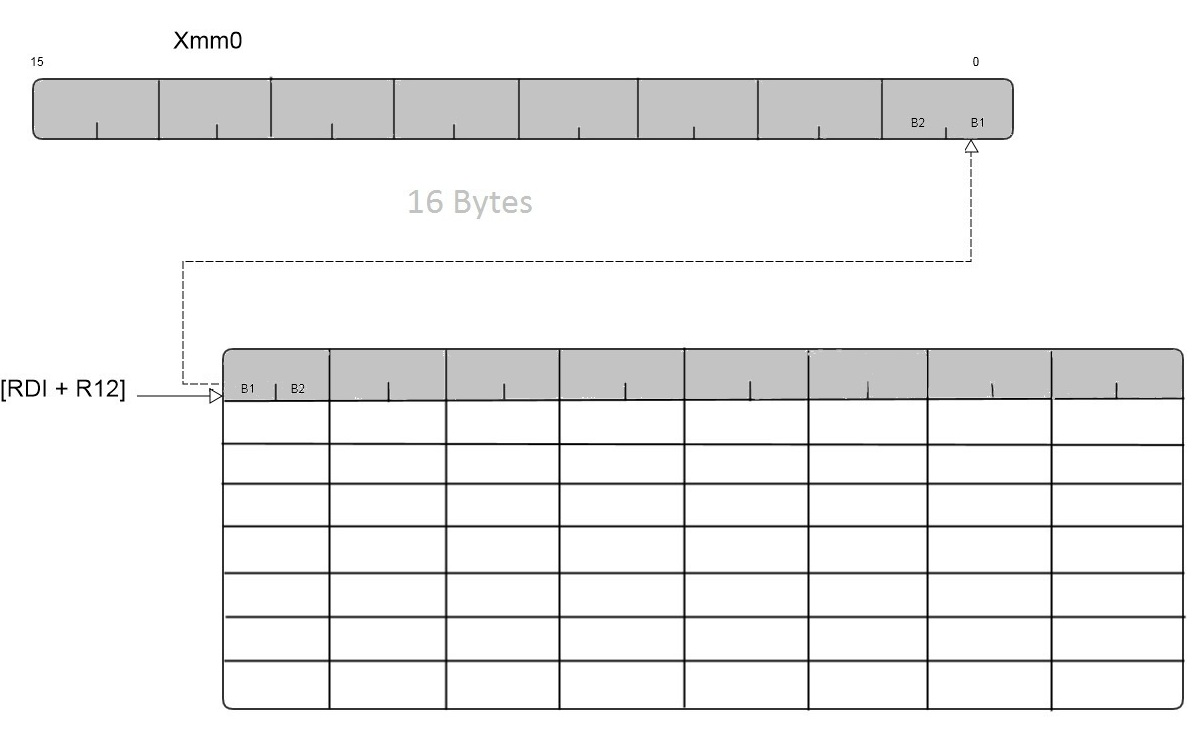
\includegraphics[height=10cm]{levantar.jpg} 

\begin{itemize}
\item Replicamos esos datos en \xmm{1}. Al hacer una operacion de conjuncion entre \xmm{1} con la mascara de \xmm{14} obtenemos los bits menos significativos de cada byte que son los codigos. Luego hacemos una nueva operacion de disyuncion logica entre \xmm{0} contra la mascara guardada en \xmm{15} y de esta forma nos quedan el tercer y cuarto bit de cada byte filtrado, que son la operacion a realizar sobre los codigos. Pero las operaciones nos quedan en el tercer y cuarto bit por eso utilizamos una intruccion de corrimiento PSRLQ para mover dos bits a la izquierda los datos obtenidos. De esta forma tenemos en \xmm{1} los codigos y en \xmm{0} los codigos de operaciones que nos dirán que modificacion realizar sobre ellos. 

Obtener codigos:

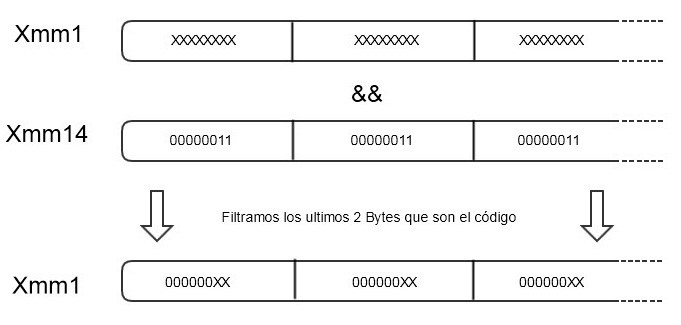
\includegraphics[height=7cm]{codigos.jpg} 

Obtener operaciones:

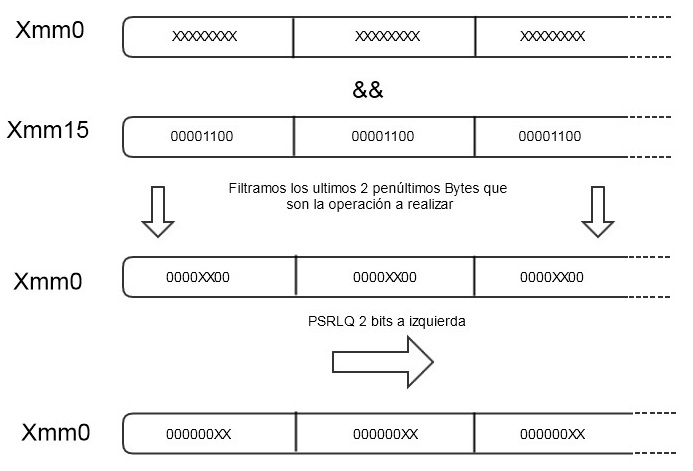
\includegraphics[height=10cm]{operaciones.jpg} 

\item Replicamos los codigos de operacion en \xmm{2}, \xmm{3} Y \xmm{4}. Paso seguido comparamos mediante la operacion PCMPEQB de comparacion empaquetada por igualdad cada registro \xmm{0}, \xmm{2}, \xmm{3} y \xmm{4} con las mascaras guardadas en los registros \xmm{10}, \xmm{11}, \xmm{12}, \xmm{13} respectivamente. Obtenemos en los registros el resultado de las comparaciones en forma de mascaras que contienen en cada posicion 0x00 y 0xFF dependiendo de si, para cada byte, en su posicion, estaba la operacion 0, 1, 2 o 3 originalmente en el registro comparado. ie. (\xmm{0} tiene 0XFF en las posiciones donde estaba la operacion 0, \xmm{2} tiene 0XFF en las posiciones donde estaba la operacion 1, etc.)

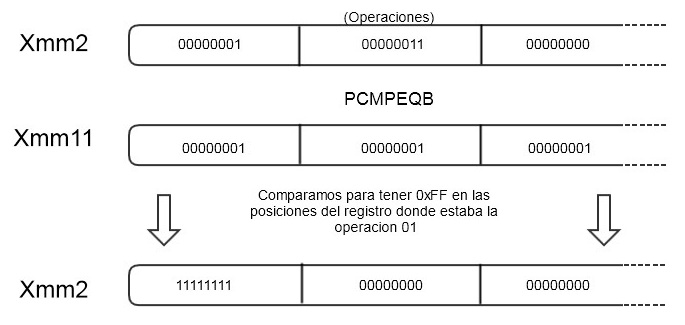
\includegraphics[height=7cm]{comparacion.jpg} 

\item En los registros \xmm{5}, \xmm{6}, \xmm{7} y \xmm{8} replico los codigos (anteriormente en \xmm{1}), y aplico a cada uno una de las operaciones a realizar sobre codigos denotadas por los codigos de operacion. Luego, para cada registro, dependiendo de la operacion que le aplique, le aplicamos una operacion logica de disyuncion contra la mascara correspondiente \xmm{0}, \xmm{2}, \xmm{3} y \xmm{4}) a los bytes en cuyo indice estaba esa operacion. De esta forma entre \xmm{5}, \xmm{6}, \xmm{7} y \xmm{8} me quedan todos los codigos con las operaciones correspondientes aplicadas y notar que los bytes empaquetados , no se superponen entre registros. De esta forma, con una conjuncion logica puedo juntar todos en un solo registro y tengo en \xmm{5} los 16 bytes que solo tienen los 2 bits mas bajos ya procesados por las operaciones.

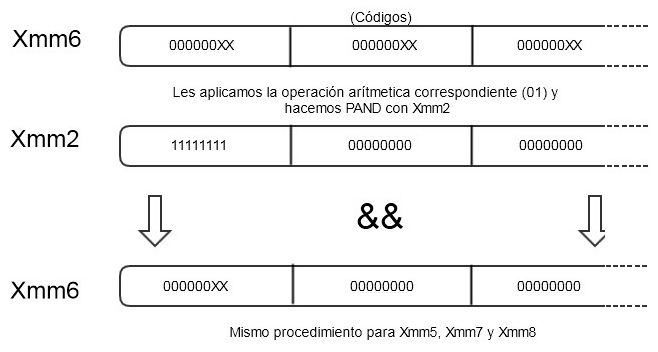
\includegraphics[height=7cm]{siguienteacomparaciones.jpg} 

Unimos resultados mediante POR's:

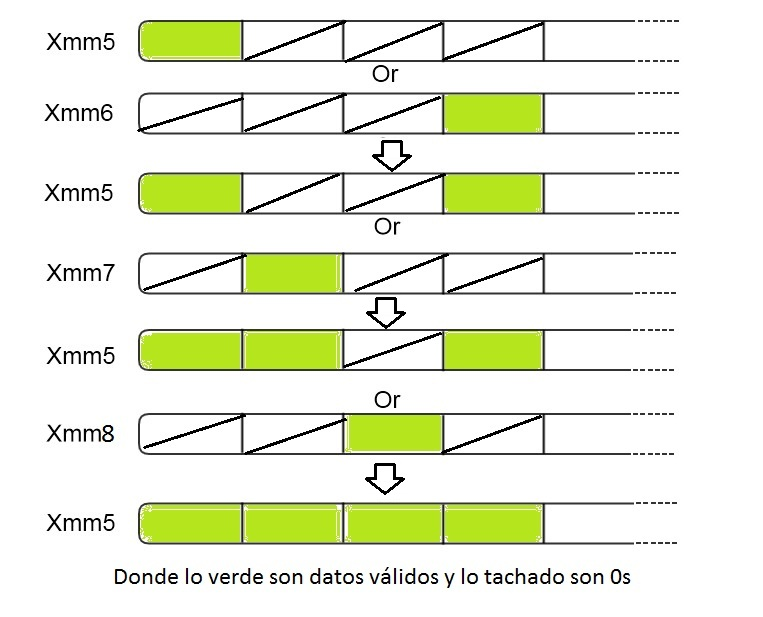
\includegraphics[height=8cm]{ors.jpg} 

\item Lo unico que queda pendiente es la combinacion de los codigos procesados para formar 4 caracteres ascii. Logramos esto mediante el uso repetido de la instruccion PEXTRB para extraer 4 bytes del registro \xmm{5}, copiarlos en \reg{8}, \reg{9}, \reg{10} y \reg{11},y realizar los corrimientos pertinentes a cada uno con el objetivo de acomodarlos en la posicion correcta y formar un byte entre todos aplicando una operacion logica de disyuncion. Esto se hace una vez por cada uno de los 4 caracteres, y la combinacion se almacena en los registros \texttt{AL}, \texttt{BL}, \texttt{CL}, \texttt{DL}

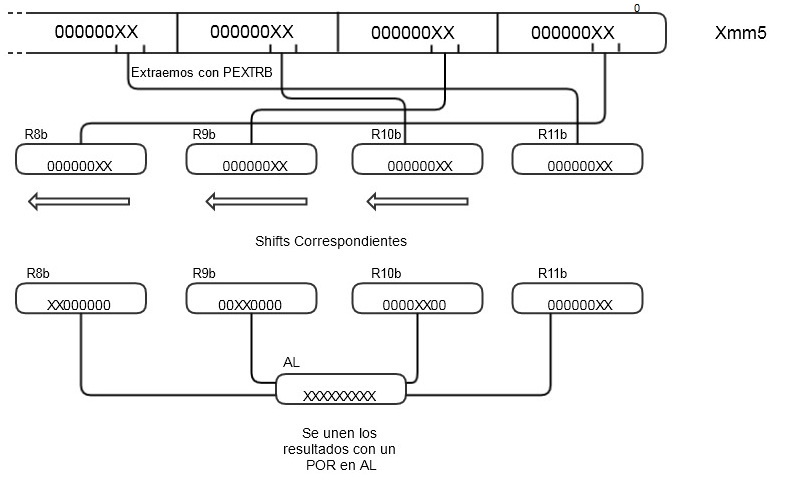
\includegraphics[height=9cm]{char.jpg} 

\item Finalmente copiamos los 4 bytes que contienen los 4 caracteres al buffer de salida. 

\end{itemize}

\subsubsection{Optimizaciones aplicadas al algoritmo}
\begin{itemize}
    \item \textbf{Implementacion de software pipelining - Ejecucion fuera de orden}
    Se implemento esta de la mejor forma a nuestro alcance tecnica para aprovechar la ejecucion fuera de orden que provee el cpu. Esto permite que instrucciones no $dependientes_{*1}$ unas de las otras sean procesadas por el cpu favoreciendo el pipeline al utilizar mas unidades de procesamiento internas de la CPU, reduciendo al minimo los stalls. Nuestra implementacion sobre el codigo assembler del filtro decode fue reorganizar las instrucciones de forma tal que el cpu pueda comenzar a ejecutar instrucciones no dependientes posteriores antes de finalizar la ejecucion de la instruccion actual. Se intento realizar la implementacion desenrrollando el ciclo en 2 procesamientos por ciclo y superponer instrucciones iguales no dependientes para lograr un mayor impacto pero abandonamos esta implementacion porque mientras nos dispusimos a realizarla, nos quedamos sin registros \xmm{} para utilizar dentro del ciclo, tal vez podriamos haber encontrado la manera de reemplazar accesos a mascaras estaticas desde registros por accesos a memoria, liberando asi mas registros, pero tomamos la decision de no hacerlo, dado que los accesos a memoria impactarian proporcionalmente al tamaño de la entrada del algoritmo y no nos parecio para nada favorable.
\end{itemize}
\par
\bigskip
\textbf{Mas info en:} \url{http://en.wikipedia.org/wiki/Software_pipelining}\\
${*1} $ \url{http://en.wikipedia.org/wiki/Hazard_(computer_architecture)}

\subsubsection{Analisis y rendimiento de las diferentes implementaciones}

La principal diferencia estructural de las dos implementaciones, es, como puede verse en los respectivos codigos, que la
implementacion en C en cada iteracion del ciclo accede a memoria y obtiene 4 bytes de forma secuencial, para luego procesarlos y obtener un caracter del texto, mientras que la implementacion en assembler se obtienen 16 bytes en cada iteracion del ciclo y son procesados paralelamente por medio instrucciones de tipo SIMD para obtener 4 caracteres por iteracion. Intuitivamente la implementacion en assembler deberia realizar 4 veces mas trabajo de procesamiento por ciclo. Todo esto sin considerar ademas temas del compilador, que no utiliza instrucciones SIMD para optimizar, realizando el procesamiento de estos datos  en forma secuencial y no paralela. \\
\\
\textbf{Nota:} La medicion se realiza sobre el metodo decode, sin tener en cuenta procesamientos externos a esta funcion, asi tambien se obtiene un promedio de la cantidad de aplicaciones de la funcion determinadas por el parametro $t$ al invocar el programa. Se probo la medicion con varios archivos provistos por la catedra, al ser de tamaño relativamente parecido, no se observaron diferencias al llevar a cabo distintos experimentos.
\\
\\
\textbf{Caracterizacion del experimento:}
\begin{itemize}
    \item \textbf{Iteraciones:} 1000
    \item \textbf{Comando:} ./tp2 -t 1000 decode -i $<implementacion>$ ../data/base/encoded.bmp 
\end{itemize}

\begin{center}
    \begin{tabular}{|l|l|l|l|}
        \hline
        Medición & Implementación C & ASM Plano & ASM Soft. Pipeline   \\
        \hline
        Ciclos por llamada &    1382837.000   & 144664.578       & 114466.883  \\
        \hline
    \end{tabular}
\end{center}
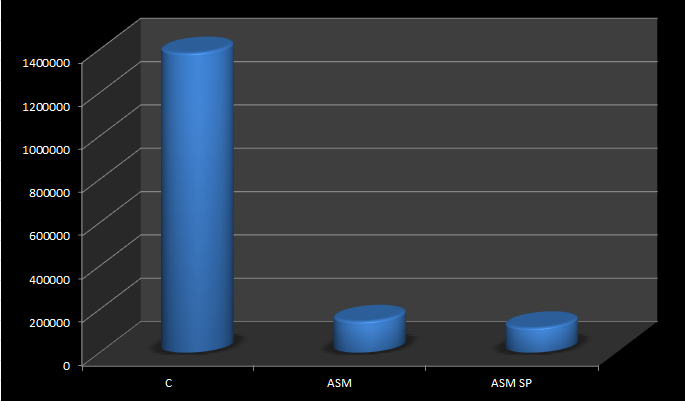
\includegraphics[scale=0.85]{imagenes/decode-resultados.png} 
\par
\bigskip
\subsubsection{Conclusiones de los resultados}
Se puede observar una mejora notable entre las versiones C y ASM, se ejecuta aproximadamente 10 veces mas rapido la version en assembler, superando las expectativas de mejora de 4 veces estimadas al comienzo de la implementacion. Asi mismo se obtuvo una mejora aproximada del $27\%$ contra el assembler original aplicando software pipelining. Lo que nos da una mejora total aproximada entre C y ASM con SP de $1200\%$



